\documentclass{ximera}

\title{What is a limit?}

\newenvironment{objectives}{\begin{remark}\textbf{Objectives}\\}{\end{remark}}

\begin{document}
\begin{abstract}
\end{abstract}

To summarize...

\begin{explanation}
    \begin{enumerate}
        \item \begin{itemize}
            \item The function $f(x)$ is continuous from the left at point $a$ if $\lim_{x \to a^-} f(x) = f(a)$
            \item The function $f(x)$ is continuous from the right at point $a$ if $\lim_{x \to a^+} f(x) = f(a)$
        \end{itemize}
        \begin{center}            
        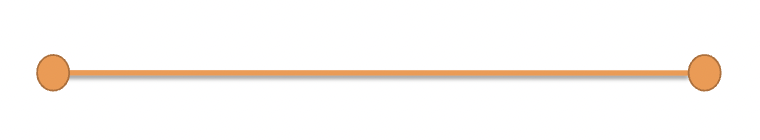
\includegraphics[width=0.5\textwidth]{graph4.png}
        \end{center}

    \item The function $f(x)$ is continuous on the open interval $(a,b)$ if it is continuous at all points of the interval

    \item The function $f(x)$ is continuous on the closed interval $[a,b]$ if it is continuous on the open interval $(a,b)$ and if $\lim_{x \to a^+} f(x) = f(a)$ and $\lim_{x \to b^-} f(x) = f(b)$.
        In other words, $f(x)$ is continuous on the closed interval $[a,b]$ if it is continuous at all points of the interior $(a,b)$, left continuous at $x=b$, and right continuous at $x=a$.
    \end{enumerate}
\end{explanation}

\end{document}